\begin{figure}[htb!]
\centering
\begin{tabular}{ll}
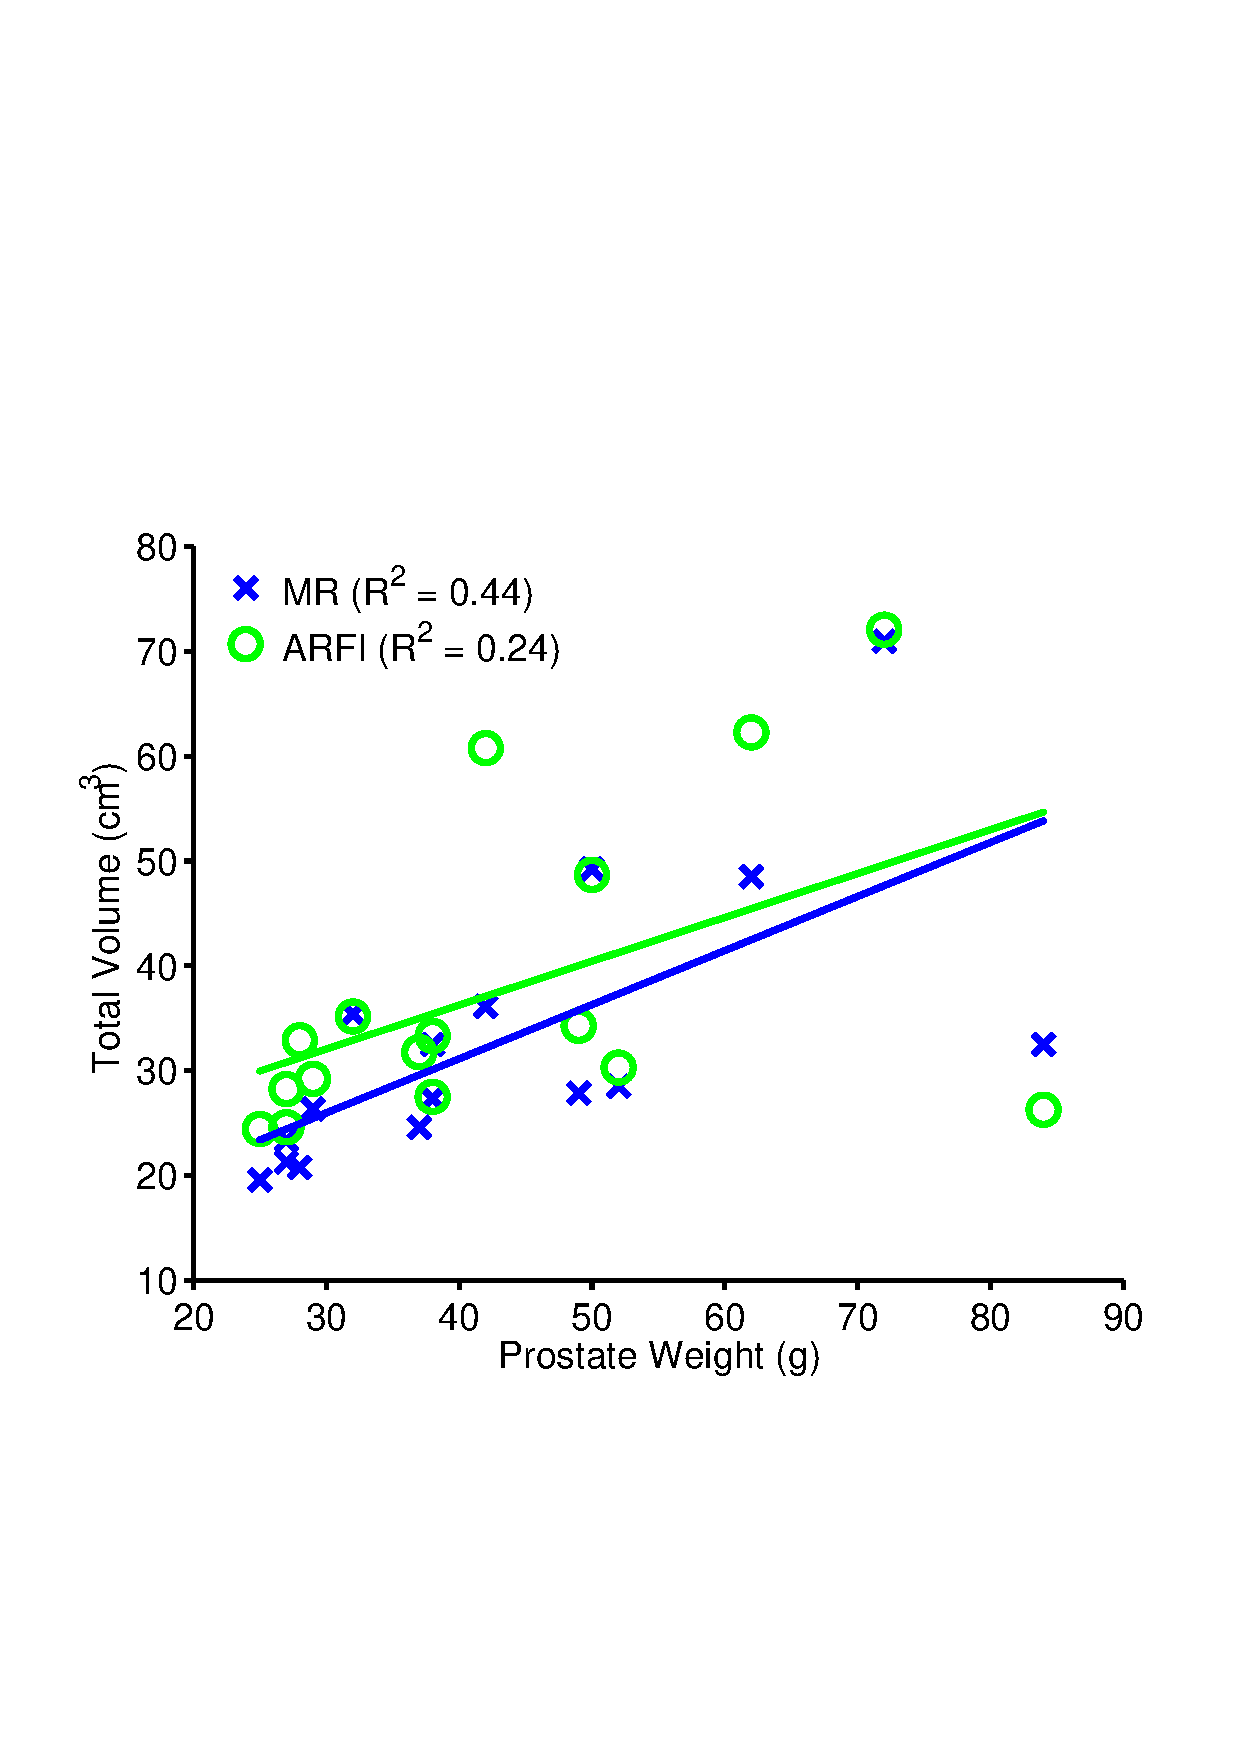
\includegraphics[width=0.33\linewidth]{figs/corr_weight_vol.pdf} &
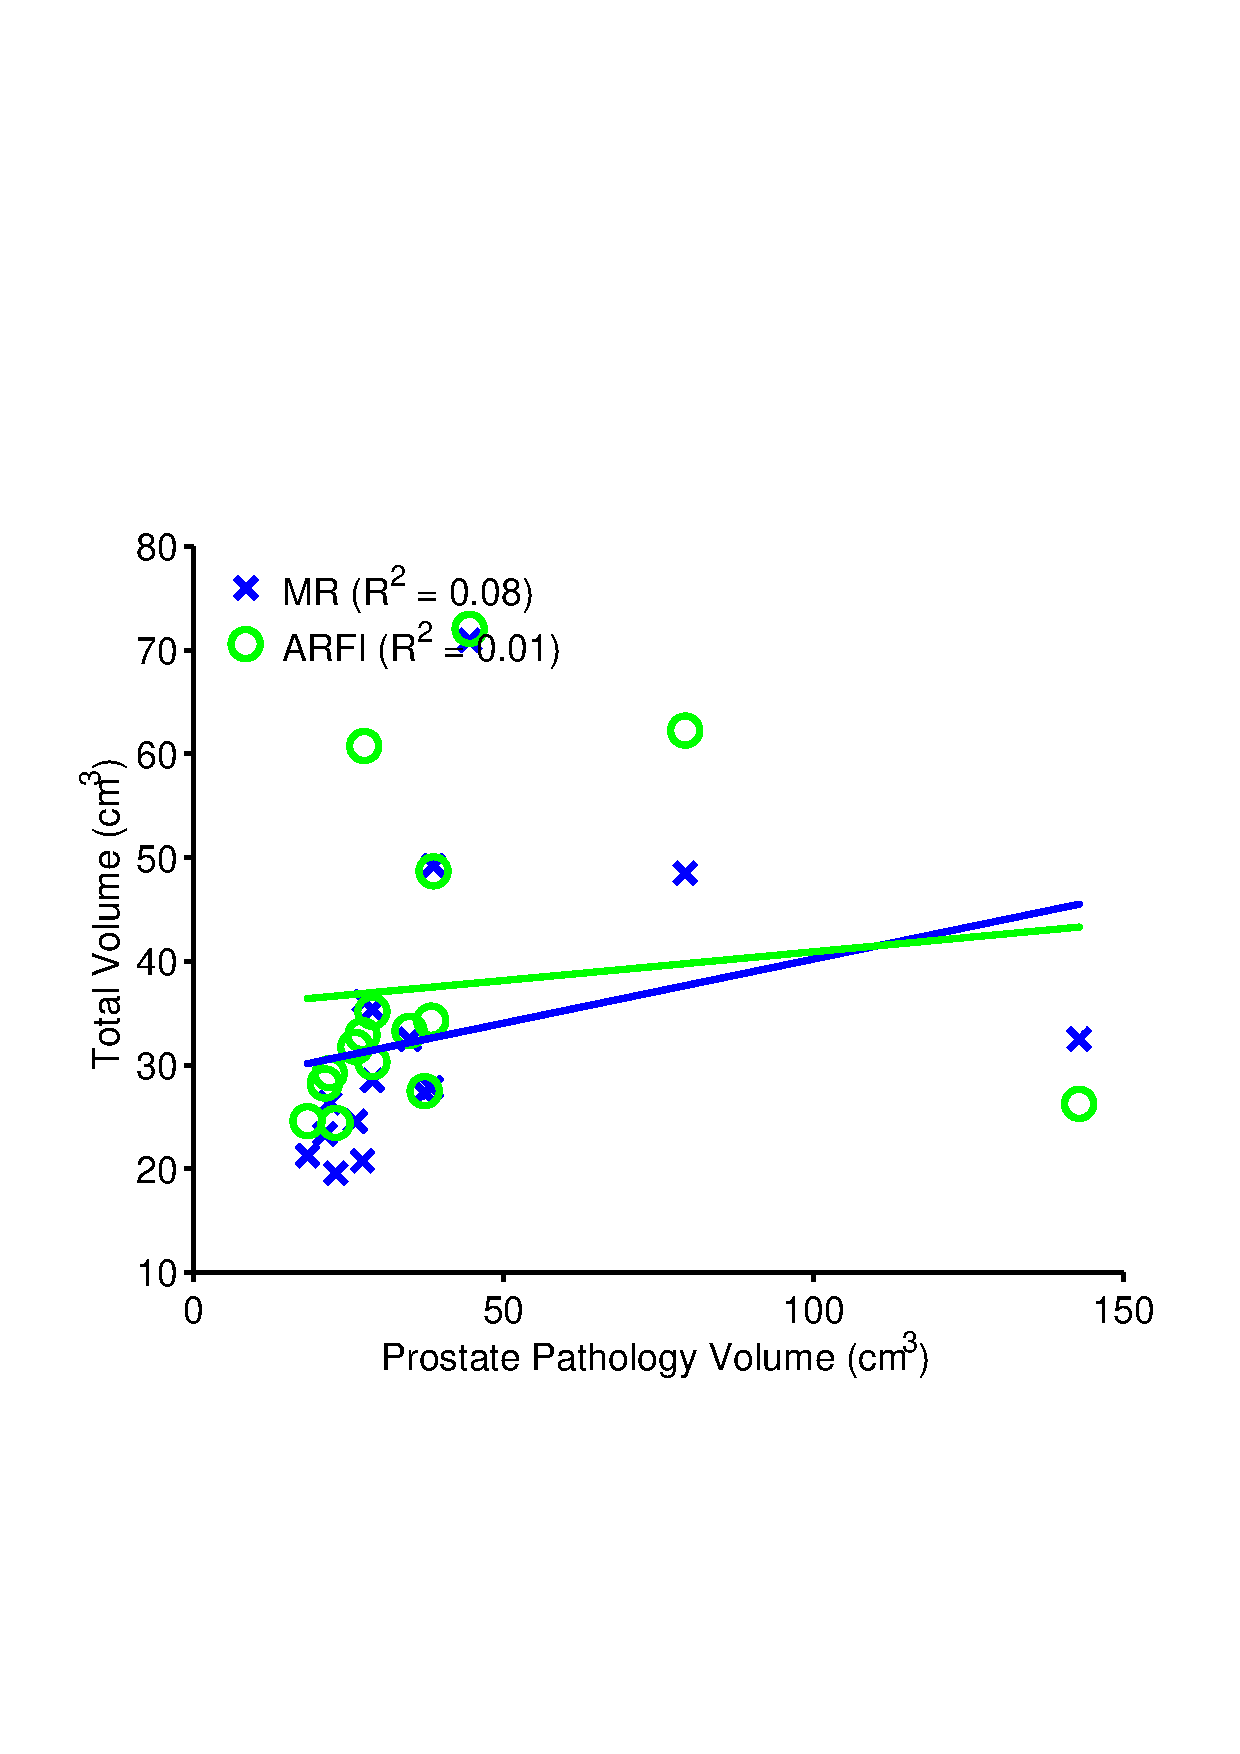
\includegraphics[width=0.33\linewidth]{figs/corr_pathVol_vol.pdf} \\
(a) Image Volume : Prostate Weight & (b) Image Volume : Pathology Volume \\
\end{tabular}
\caption{The prostates analyzed in this study showed no significant correlation
    between their measured excised pathology weight (a) and the reconstructed
    volumes in T2WI MR (blue) and ARFI imaging (green).  The coefficients of
    determination (R$^2$) for the linear regressions for each imaging modality
    were 0.05 and 0.13, respectively, indicating no significant correlation.
    Tri-axial pathology measurements were used to make an ellipsoidal prostate
    volume approximation (b), which showed mild correlation with T2WI MR (R$^2$
    = 0.32) and moderate correlation with ARFI imaging (R$^2$ = 0.71).}
\label{fig:mr_arfi_weight} 
\end{figure}
